%%%%%%%%%%%%%%%%%%%%%%%%%%%%%%%%%%%%%%%%%
% Wenneker Assignment
% LaTeX Template
% Version 2.0 (12/1/2019)
%
% This template originates from:
% http://www.LaTeXTemplates.com
%
% Authors:
% Vel (vel@LaTeXTemplates.com)
% Frits Wenneker
%
% License:
% CC BY-NC-SA 3.0 (http://creativecommons.org/licenses/by-nc-sa/3.0/)
%
%%%%%%%%%%%%%%%%%%%%%%%%%%%%%%%%%%%%%%%%%

%----------------------------------------------------------------------------------------
%	PACKAGES AND OTHER DOCUMENT CONFIGURATIONS
%----------------------------------------------------------------------------------------

\documentclass[11pt]{article} % Font size
\usepackage{comment}
\usepackage{color}
%%%%%%%%%%%%%%%%%%%%%%%%%%%%%%%%%%%%%%%%%
% Wenneker Assignment
% Structure Specification File
% Version 2.0 (12/1/2019)
%
% This template originates from:
% http://www.LaTeXTemplates.com
%
% Authors:
% Vel (vel@LaTeXTemplates.com)
% Frits Wenneker
%
% License:
% CC BY-NC-SA 3.0 (http://creativecommons.org/licenses/by-nc-sa/3.0/)
% 
%%%%%%%%%%%%%%%%%%%%%%%%%%%%%%%%%%%%%%%%%

%----------------------------------------------------------------------------------------
%	PACKAGES AND OTHER DOCUMENT CONFIGURATIONS
%----------------------------------------------------------------------------------------

\usepackage{amsmath, amsfonts, amsthm} % Math packages
\usepackage{tabto}
\usepackage{listings} % Code listings, with syntax highlighting
\usepackage{tabu}
\usepackage{array}
\usepackage[english]{babel} % English language hyphenation
\usepackage{hyperref}

\usepackage{graphicx} % Required for inserting images
\graphicspath{{Figures/}{./}} % Specifies where to look for included images (trailing slash required)

\usepackage{booktabs} % Required for better horizontal rules in tables

\numberwithin{equation}{section} % Number equations within sections (i.e. 1.1, 1.2, 2.1, 2.2 instead of 1, 2, 3, 4)
\numberwithin{figure}{section} % Number figures within sections (i.e. 1.1, 1.2, 2.1, 2.2 instead of 1, 2, 3, 4)
\numberwithin{table}{section} % Number tables within sections (i.e. 1.1, 1.2, 2.1, 2.2 instead of 1, 2, 3, 4)

\setlength\parindent{0pt} % Removes all indentation from paragraphs

\usepackage{enumitem} % Required for list customisation
\setlist{noitemsep} % No spacing between list items

%----------------------------------------------------------------------------------------
%	DOCUMENT MARGINS
%----------------------------------------------------------------------------------------

\usepackage{geometry} % Required for adjusting page dimensions and margins

\geometry{
	paper=a4paper, % Paper size, change to letterpaper for US letter size
	top=2.5cm, % Top margin
	bottom=3cm, % Bottom margin
	left=3cm, % Left margin
	right=3cm, % Right margin
	headheight=0.75cm, % Header height
	footskip=1.5cm, % Space from the bottom margin to the baseline of the footer
	headsep=0.75cm, % Space from the top margin to the baseline of the header
	%showframe, % Uncomment to show how the type block is set on the page
}

%----------------------------------------------------------------------------------------
%	FONTS
%----------------------------------------------------------------------------------------

\usepackage[utf8]{inputenc} % Required for inputting international characters
\usepackage[T1]{fontenc} % Use 8-bit encoding

\usepackage{fourier} % Use the Adobe Utopia font for the document

%----------------------------------------------------------------------------------------
%	SECTION TITLES
%----------------------------------------------------------------------------------------

\usepackage{sectsty} % Allows customising section commands

\sectionfont{\vspace{6pt}\centering\normalfont\scshape} % \section{} styling
\subsectionfont{\normalfont\bfseries} % \subsection{} styling
\subsubsectionfont{\normalfont\itshape} % \subsubsection{} styling
\paragraphfont{\normalfont\scshape} % \paragraph{} styling

%----------------------------------------------------------------------------------------
%	HEADERS AND FOOTERS
%----------------------------------------------------------------------------------------

\usepackage{scrlayer-scrpage} % Required for customising headers and footers

\ohead*{} % Right header
\ihead*{} % Left header
\chead*{} % Centre header

\ofoot*{} % Right footer
\ifoot*{} % Left footer
\cfoot*{\pagemark} % Centre footer
 % Include the file specifying the document structure and custom commands
\usepackage{graphicx}
\usepackage{subcaption}




%Code retrieved from: https://www.overleaf.com/project/5c52d66b6343590b46b4fd03


%----------------------------------------------------------------------------------------
%	TITLE SECTION
%----------------------------------------------------------------------------------------

\title{
	\normalfont\normalsize
	\textsc{Old Dominion University}\\ % Your university, school and/or department name(s)
	\vspace{25pt} % Whitespace
	\rule{\linewidth}{0.5pt}\\ % Thin top horizontal rule
	\vspace{20pt} % Whitespace
	{\huge Assignment 5}\\ % The assignment title
	\vspace{12pt} % Whitespace
	\rule{\linewidth}{2pt}\\ % Thick bottom horizontal rule
	\vspace{12pt} % Whitespace
}

\author{\LARGE David Bayard} % Your name

\date{\normalsize\today} % Today's date (\today) or a custom date

\begin{document}

\definecolor{codegreen}{rgb}{0,0.6,0}
\definecolor{codegray}{rgb}{0.5,0.5,0.5}
\definecolor{codepurple}{rgb}{0.58,0,0.82}
\definecolor{backcolour}{rgb}{0.95,0.95,0.92}
\lstdefinestyle{pythonStyle}{
  backgroundcolor=\color{backcolour},
  commentstyle=\color{codegreen},
  keywordstyle=\color{magenta},
  numberstyle=\tiny\color{codegray},
  stringstyle=\color{codepurple},
  basicstyle=\footnotesize,
  breakatwhitespace=false,
  breaklines=true,
  captionpos=b,
  keepspaces=true,
  numbers=left,
  numbersep=5pt,
  showspaces=false,
  showstringspaces=false,
  showtabs=false,
  tabsize=2
}

\lstset{style=pythonStyle}


\maketitle % Print the title

\pagebreak
\section*{Question 1.}



%------------------------------------------------

\subsection*{We know the result of the Karate Club (Zachary, 1977) split.
Prove or disprove that the result of split could have been predicted
by the weighted graph of social interactions.  How well does the
mathematical model represent reality?}
\bigskip\bigskip


\Large Solution:
\newline \newline\small

\tabto{2.0cm} This paper will demonstrate that a mathematical model or algorith, Girvan Newman in this case, could have been used to predict the results of the Karate Club split. \newline \newline

\tabto{2.0cm} To start off, a description of the Girven Newman alrorithm must be provided. In simplest terms, the Girven Newman alrogith works by finding the edge with the highest central betweenness. This edge is then removed, and the central betweenness of each edge is recalculated. This process is repeated until two separate components are recognized. There is a library in Python called networkx, which provides functions that find the highest central edge betweenness, and remove specific edges, among other things. This library was used to graph the Karate Club before the split, and to iteratively remove edges from the Karate Club graph. \newline \newline

In more formal terms, the formula to calculate the central edge betweenness for the vertex is: $$ C_ B (v) = \sum _{(s\neq v \neq \ t \epsilon V) } \frac {\sigma_{st} (v)}{\sigma{st}} $$

Where $ \sigma_{st}$ is the total number of shortest paths from node s to node t and $\sigma_{st}(v)$ is the number of those paths that pass through v. 
\newline \newline
\tabto{2.0cm} This formula provides access to the edge with the higest betweenness, which will be removed repeatedly to disconnect the communities in the graph. The functions used to calculate the central edge betweenness and remove the edge are displayed below, as well as a sorting method. This is used to obtain the element with the highest central betweenness value, rather then the one with the lowest edge betweenness.  \newline \newline
\begin{lstlisting}[language = Python, caption=Finding central edge betweenness]
 eb = nx.edge_betweenness_centrality(G0)
    
    sortedDict = (sorted(eb.items(), key=lambda key: key[1], reverse=True))

    
    return sortedDict[0][0]

\end{lstlisting} \bigskip 

\tabto{2.0cm} Once the edge with the highest betweenness value found, a function is called to remove the edge, and this is repeated until the graph is split into two communities. This mimics the real life Karate Club split because an edge between any two nodes represents an association between two members of the Karate Club, whom interact outside of the club. As a result, the graph contains nodes and edges which represent club members, and the people whom they directly interact with. Thus, removing the edge with the highest betweenness is representative of removing the individual whom was most involved in both Mr.Hi's group and John. A's group. The code to split the communities is shown below:

\begin{lstlisting}[language = Python, caption=Extracting Friend Count]
while sum(1 for x in components) == 1:
    
    # Remove Original Node
    formattedGraph.remove_edge(*find_best_edge(formattedGraph))
    
    components = nx.connected_component_subgraphs(formattedGraph)

  plt.show()

  result = [c.nodes() for c in components]
  
  for c in components: 
    result.extend(girvan_newman(c))
\end{lstlisting}

On pages 4 and 5, images displaying the removal of edges with the higest central betweenness values are displayed. The first image represents the orginal Karate Club Graph, where each node represents a person in the Karate Club. For the case of this example, node 0 will represent Mr. Hi, and node 33 represents the president of the Karate Club, John A. Every node is connected by an edge, which, as stated earlier, represent an association between two nodes, or people, outside of the Karate Club. 

\begin{figure}[h!]
\begin{center}
\begin{subfigure}[b]{.6\linewidth }
    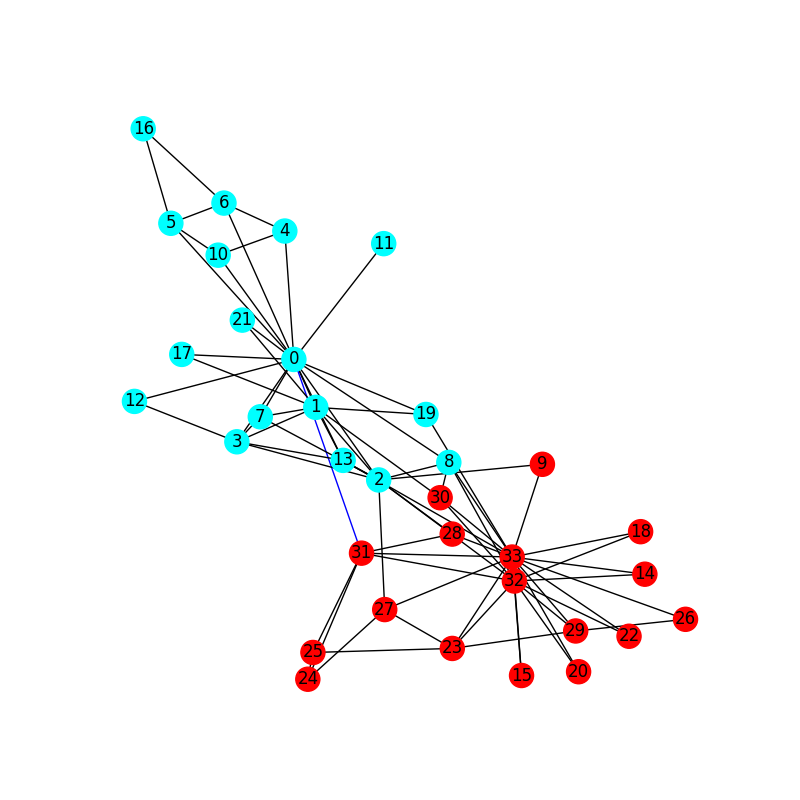
\includegraphics[width=\linewidth]{../Figures/Iteration1.png}
    \caption{Initial Graph}
\end{subfigure}
\end{center}
\end{figure}

\tabto{2.0cm} The graph above is the first representation of the Karate Club graph before the Girvan-Newman method is graphed. In this illustration, there is an edge colored in blue, which is the edge with the highest central betweenness value. This edge will be removed, and a new graph will be constructed, and this process will be repeated until two the two seperate communities are formed. This graph is produced using the networkx function below.

\begin{lstlisting}[language = Python, caption=Karate Club Graph]
 G=nx.karate_club_graph()
\end{lstlisting} \bigskip 


\begin{figure}[h!]
  \centering
  \begin{subfigure}[b]{0.4\linewidth}
    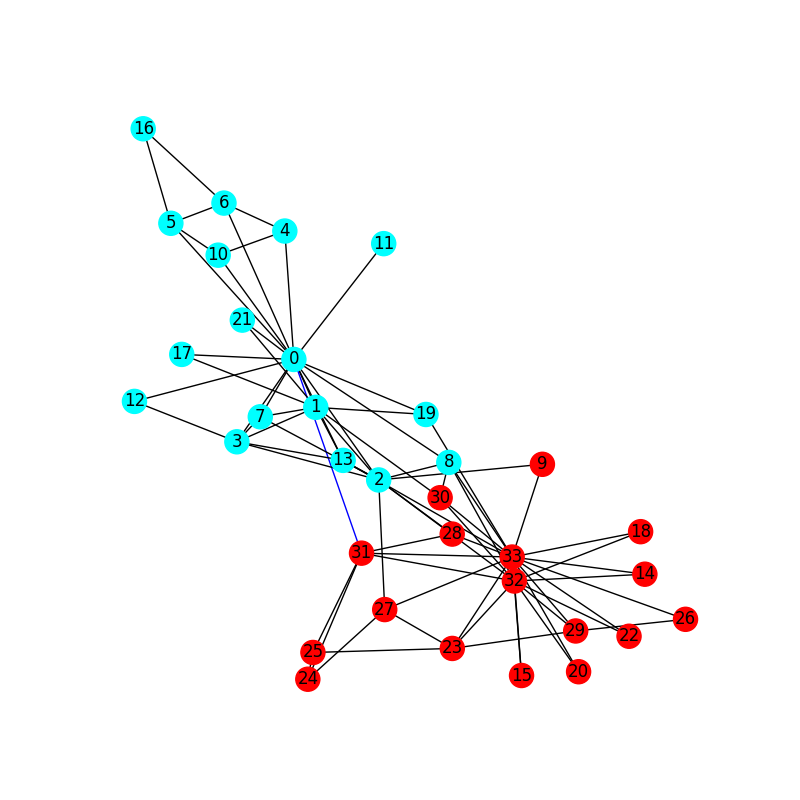
\includegraphics[width=\linewidth]{../Figures/Iteration1.png}
    \caption{Iteration 1}
  \end{subfigure}
  \begin{subfigure}[b]{0.4\linewidth}
    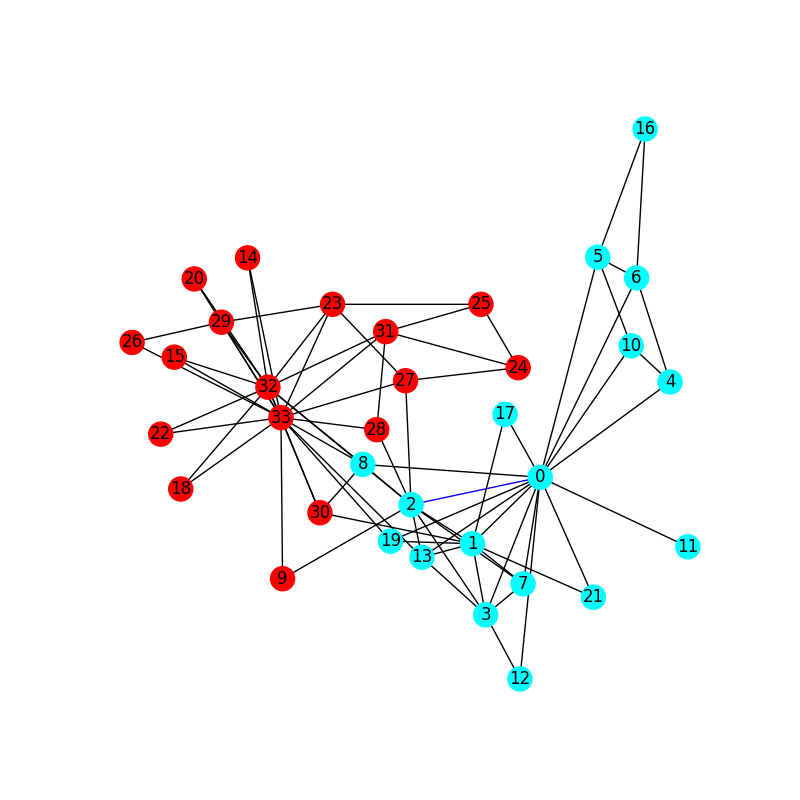
\includegraphics[width=\linewidth]{../Figures/Iteration2.png}
    \caption{Iteration 2}
  \end{subfigure}
  \begin{subfigure}[b]{0.4\linewidth}
    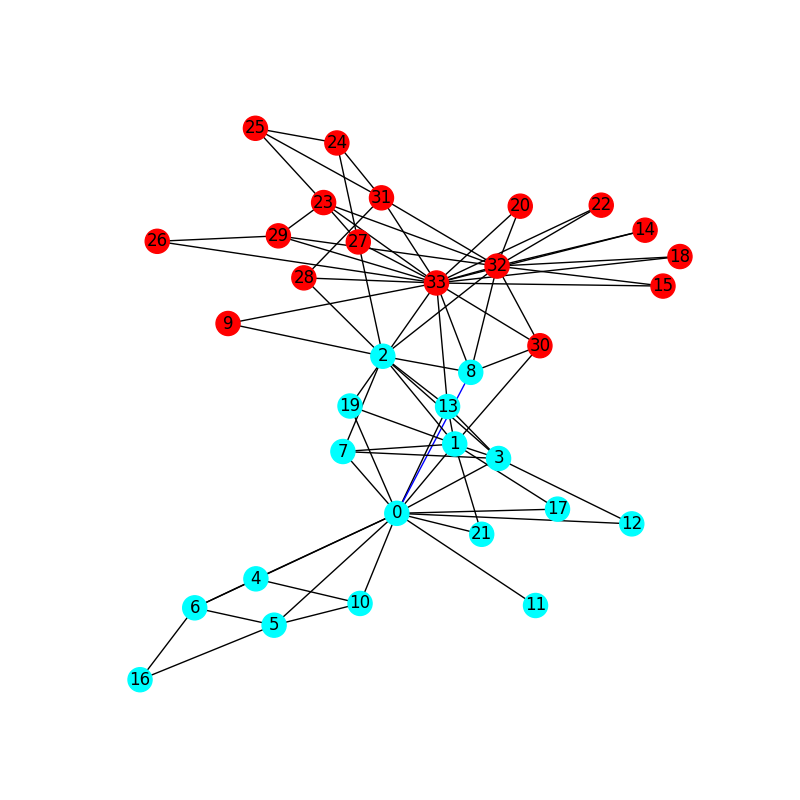
\includegraphics[width=\linewidth]{../Figures/Iteration3.png}
    \caption{Iteration 3}
  \end{subfigure}
  \begin{subfigure}[b]{0.4\linewidth}
    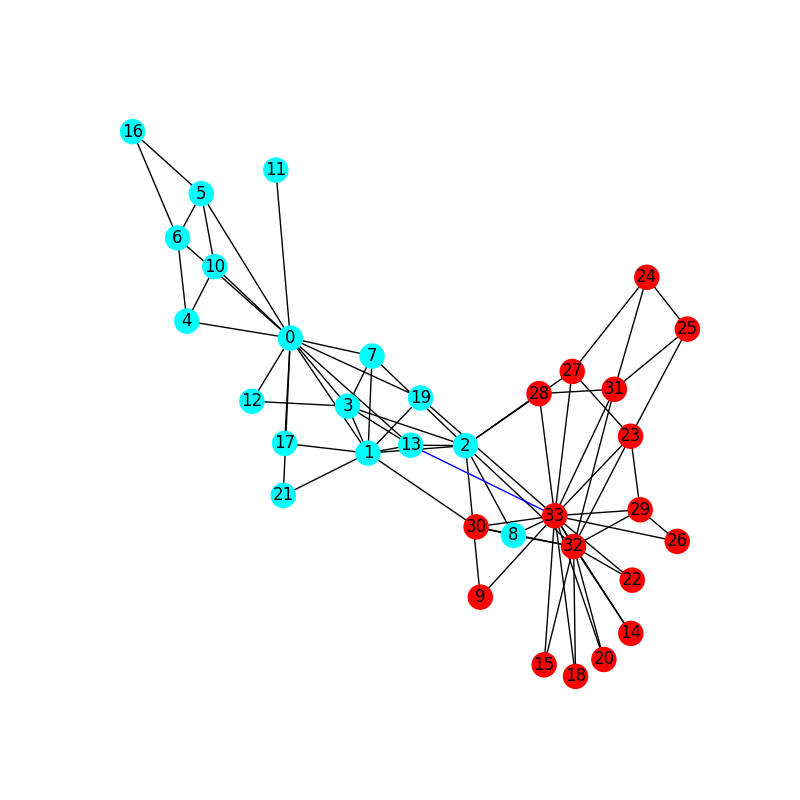
\includegraphics[width=\linewidth]{../Figures/Iteration4.png}
    \caption{Iteration 4}
  \end{subfigure}
  \begin{subfigure}[b]{0.4\linewidth}
    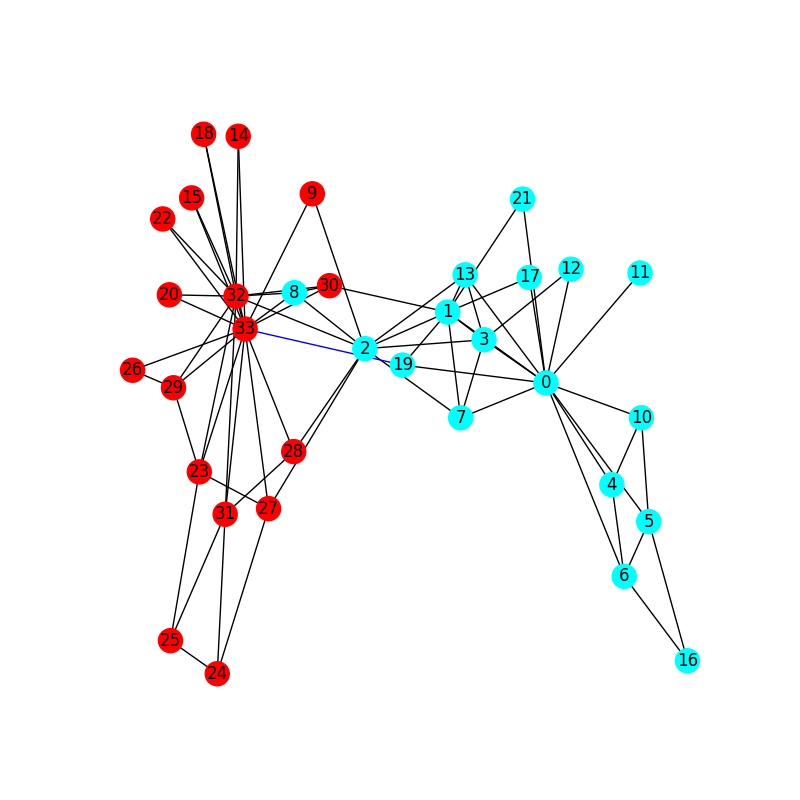
\includegraphics[width=\linewidth]{../Figures/Iteration5.png}
    \caption{Iteration 5}
  \end{subfigure}
  \begin{subfigure}[b]{0.4\linewidth}
    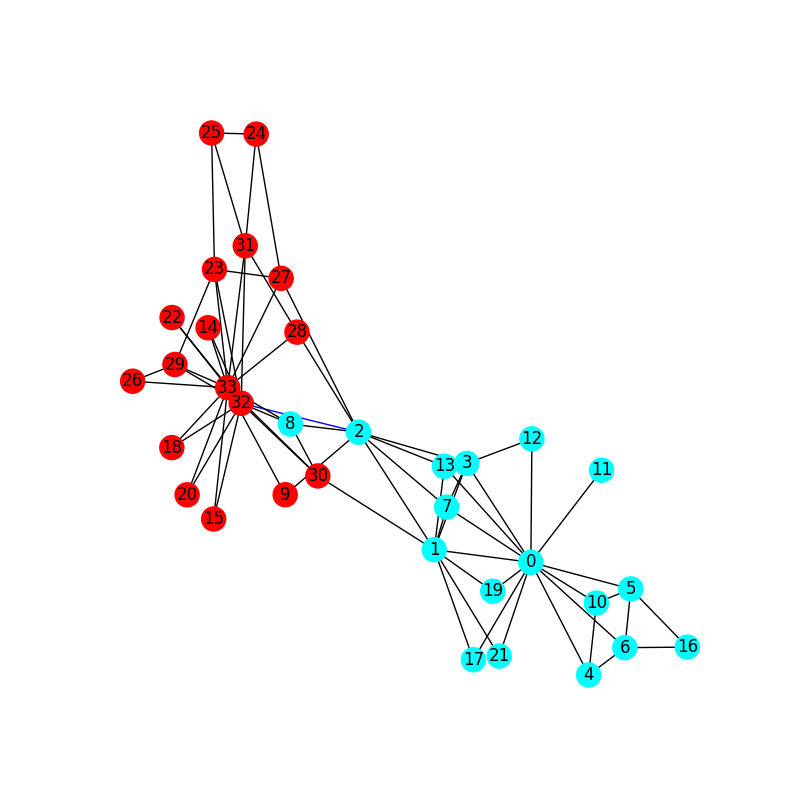
\includegraphics[width=\linewidth]{../Figures/Iteration6.png}
    \caption{Iteration 6}
  \end{subfigure}
  \caption{Splitting Graph Part1}
  \label{../Figures/Iteration1.png}
\end{figure}
\clearpage %force a page break

\begin{figure}[h!]
  \centering
  \begin{subfigure}[b]{0.4\linewidth}
    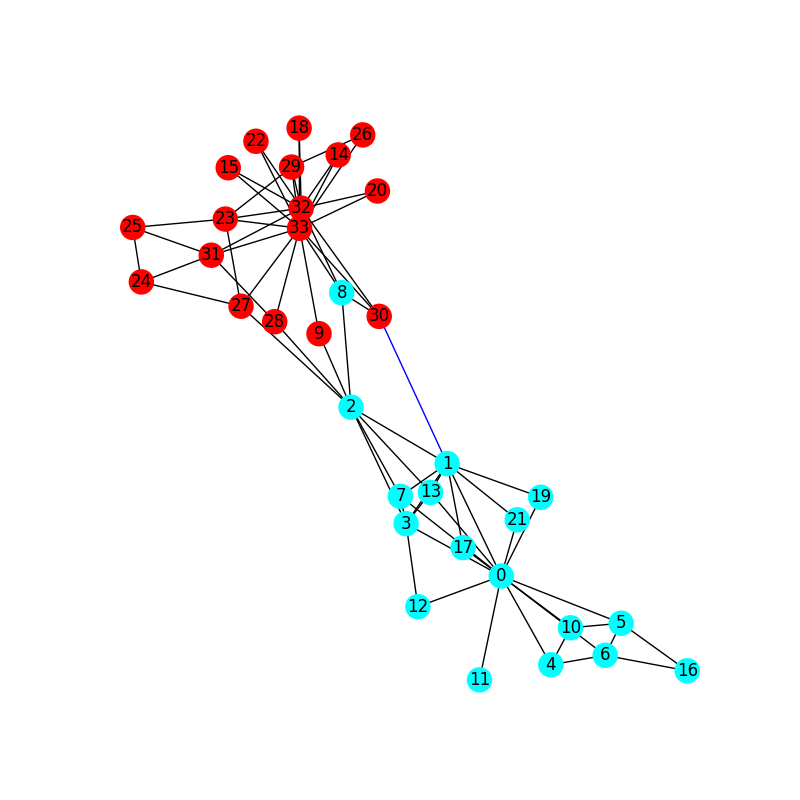
\includegraphics[width=\linewidth]{../Figures/Iteration7.png}
    \caption{Iteration 7}
  \end{subfigure}
\begin{subfigure}[b]{0.4\linewidth}
    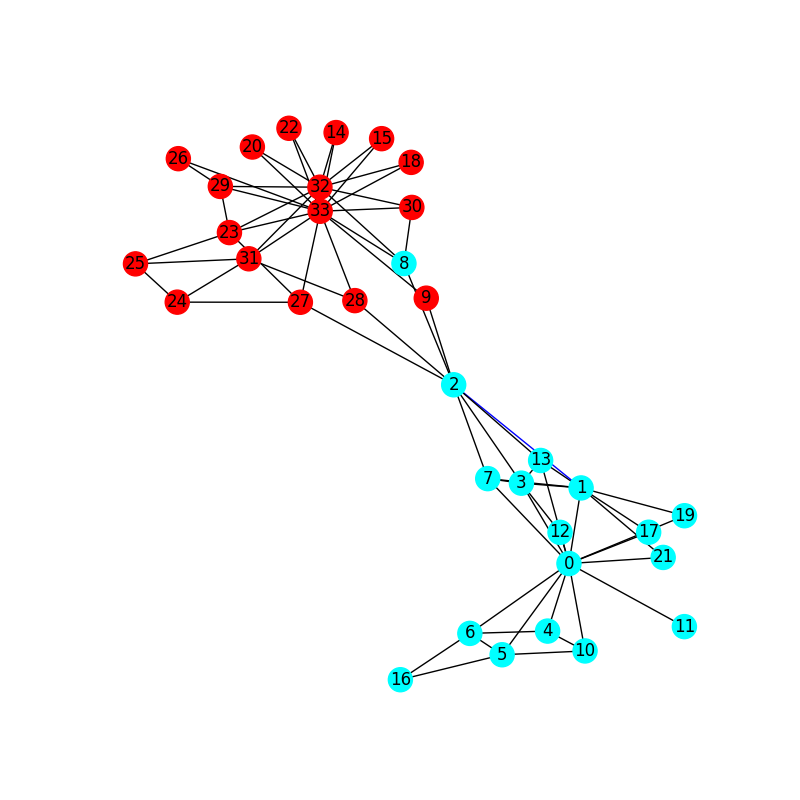
\includegraphics[width=\linewidth]{../Figures/Iteration8.png}
    \caption{Iteration 8}
  \end{subfigure}
  \begin{subfigure}[b]{0.4\linewidth}
    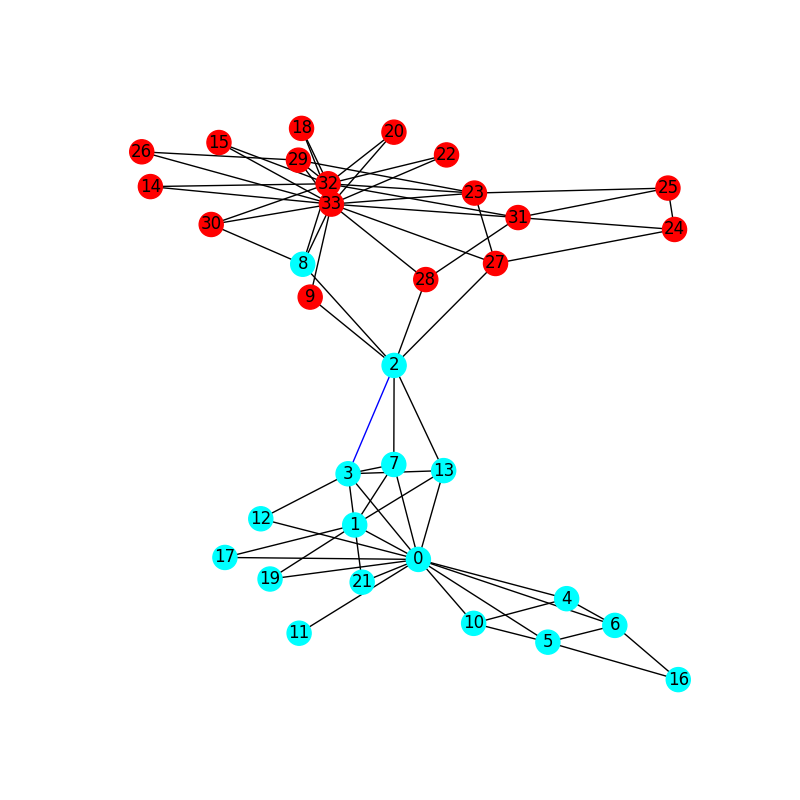
\includegraphics[width=\linewidth]{../Figures/Iteration9.png}
    \caption{Iteration 9}
  \end{subfigure}
  \begin{subfigure}[b]{0.4\linewidth}
    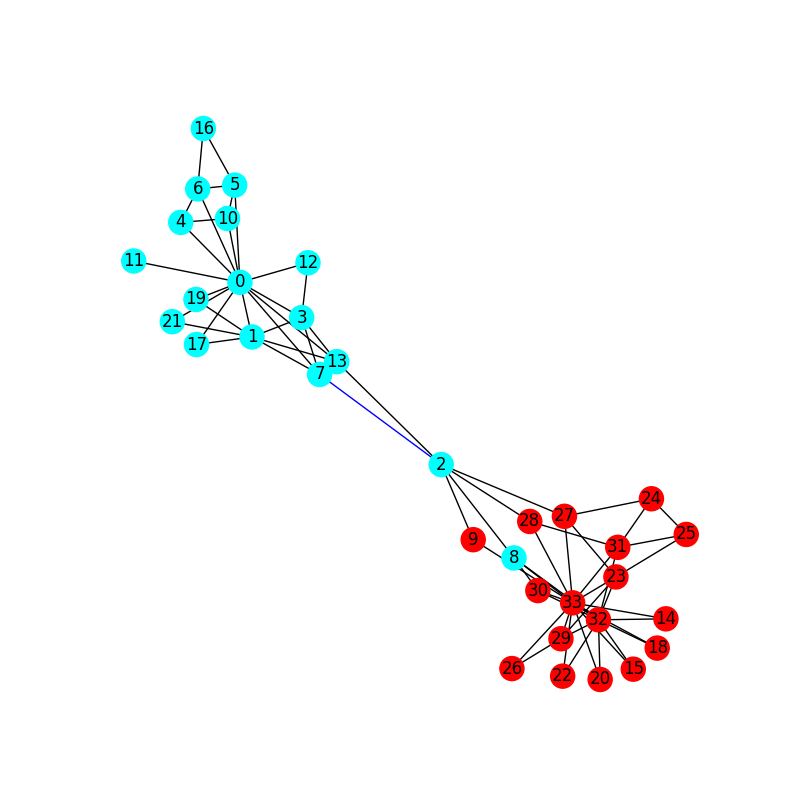
\includegraphics[width=\linewidth]{../Figures/Iteration10.png}
    \caption{Iteration 10}
  \end{subfigure}
  \begin{subfigure}[b]{0.4\linewidth}
    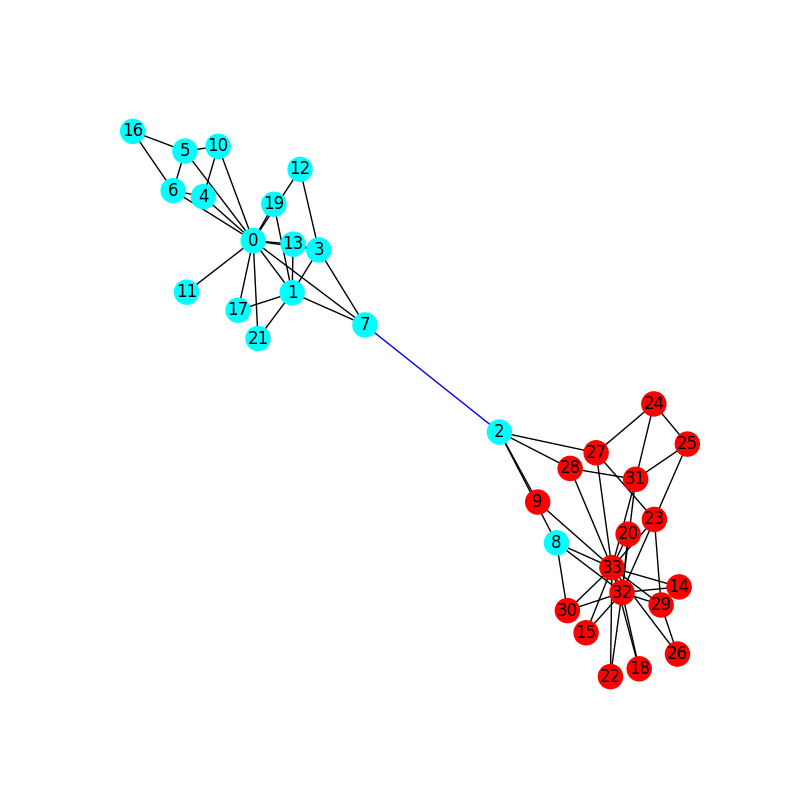
\includegraphics[width=\linewidth]{../Figures/Iteration11.png}
    \caption{Iteration 11}
  \end{subfigure}
  \begin{subfigure}[b]{0.4\linewidth}
    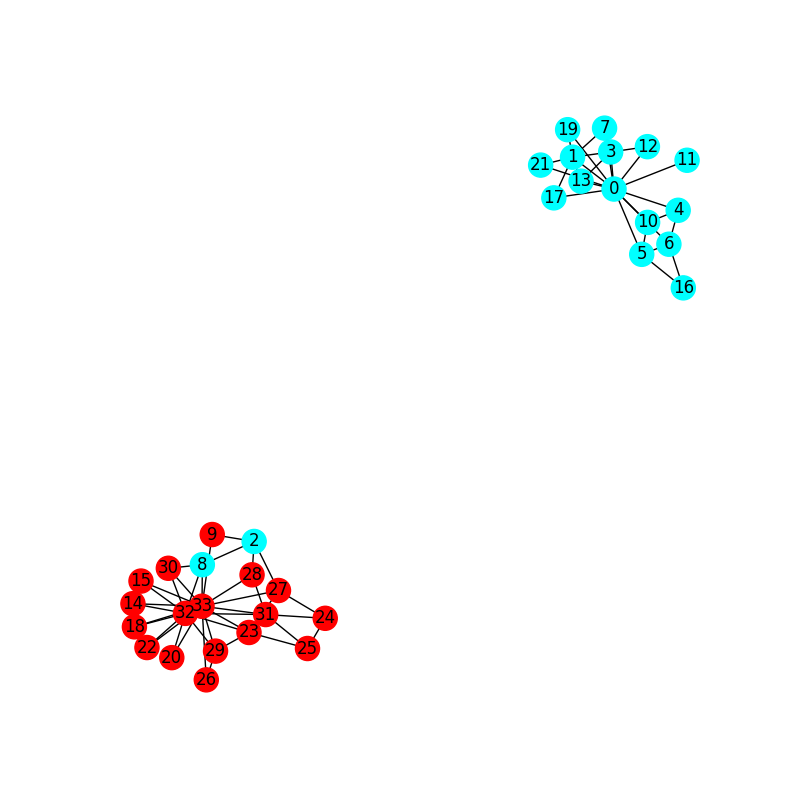
\includegraphics[width=\linewidth]{../Figures/SplitComponents.png}
    \caption{Fully Split}
  \end{subfigure}
\caption{Splitting Graph Part 2}
  \label{../Figures/Iteration1.png}
\end{figure}

\pagebreak

\tabto{2.0cm} By examining the final product, which display the split communities, it is evident that the graph could have been used to predict the Karate Club split. This evident, because the final graph only differs from the real Karate Club split with regards to node 2. This node should belong to Mr.Hi's group, but instead exists within John A's group. With only this point of infliction, the Girvan-Newman algorithm provides 33 correct predictments out of 34. This results in 97\% of the predictions being accurate, concluding that it is indeed possible to predict the Karate Club split with marginal error.

\clearpage
\section*{Question 3. Extra Credit}


\subsection*{We know the group split in two different groups.  Suppose the
disagreements in the group were more nuanced -- what would the clubs
look like if they split into groups of 3, 4, and 5?}
\bigskip\bigskip


\Large Solution:
\newline \newline\small

\tabto{2.0cm} This is determined by running the Girvan-Newman algorithm until the community breaks into 3, 4, and 5 respective communities. The same process will be repeated from splitting the same communities, which will provide an accurate representation of the club after the splits.

\begin{figure}[h!]
  \centering
  \begin{subfigure}[b]{0.5\linewidth}
    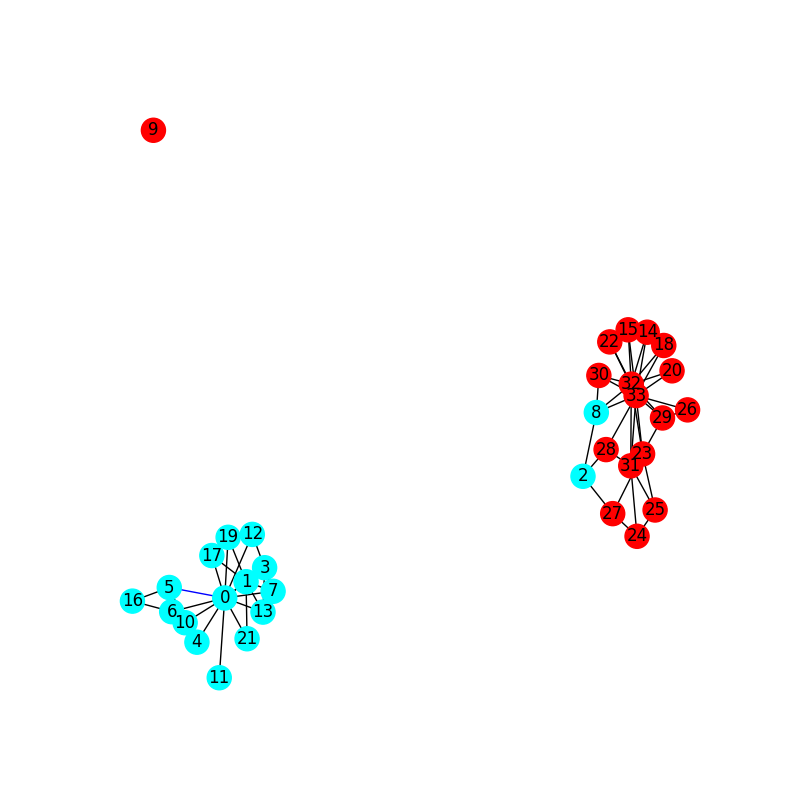
\includegraphics[width=\linewidth]{../Figures/3_communities.png}
    \caption{3 Groups}
  \end{subfigure}
\begin{subfigure}[b]{0.5\linewidth}
    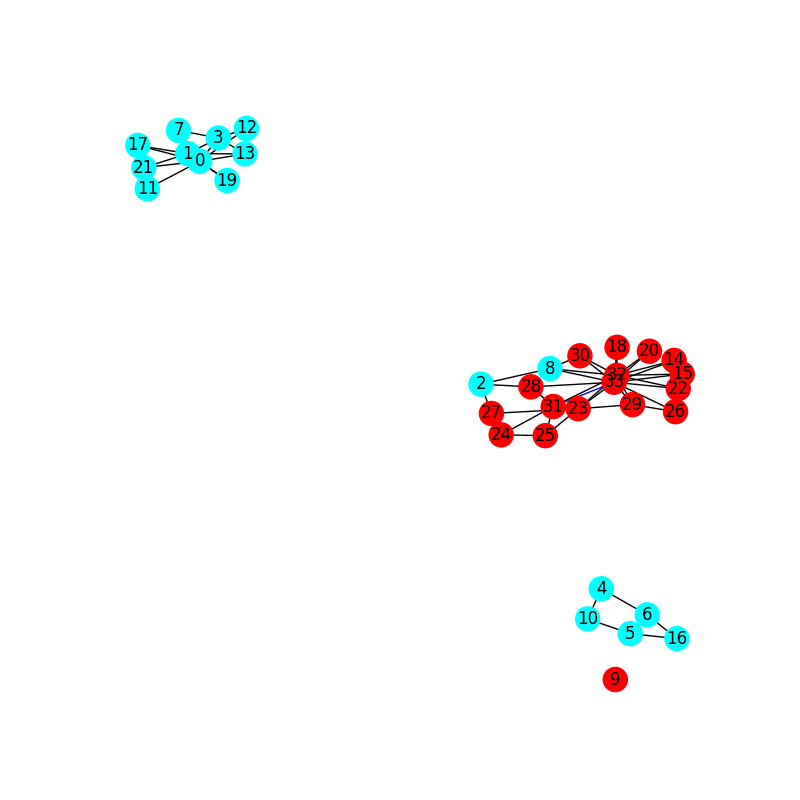
\includegraphics[width=\linewidth]{../Figures/4_communities.png}
    \caption{4 Groups}
  \end{subfigure}
  \begin{subfigure}[b]{0.5\linewidth}
    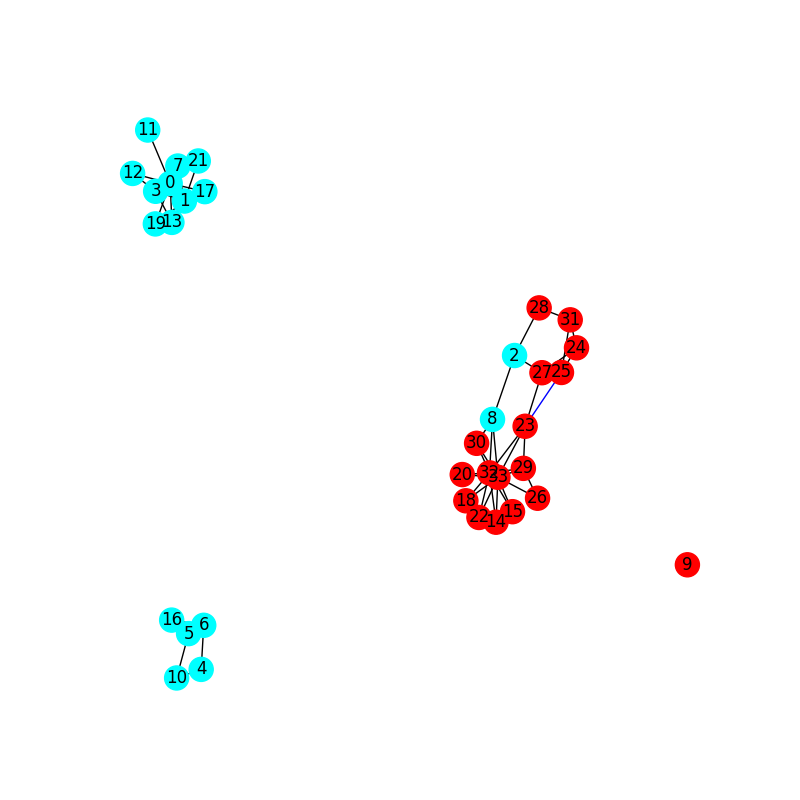
\includegraphics[width=\linewidth]{../Figures/5_communities.png}
    \caption{5 Groups}
  \end{subfigure}
\caption{Graphs for groups 3, 4, and 5}
  \label{../Figures/Iteration1.png}
\end{figure}

\end{document}
